% -------------------------------------------------------------------------------------- %

\documentclass[letterpaper,10pt]{article}



\pagestyle{empty}

\usepackage[table]{xcolor}
\usepackage{color, colortbl}
\usepackage{tabularx}
\usepackage{amssymb}
\usepackage{enumerate}

\definecolor{LightGray}{gray}{0.9}

\usepackage{amsmath}
\usepackage{amscd}
\usepackage{url}

\usepackage{graphicx}


\title{Installing AIMBAT}
\author{Seismo Group}
\date{\today}

\begin{document}
\maketitle

% ************************************************************* %
%                                                               %
%                       OPERATING SYSTEM                        %
%                                                               %
% ************************************************************* %

\section{Getting your Operating System}

Go to \verb"System Preferences" as in~\ref{fig:system_preferences}, and click on \verb"Startup Disk". It should show your operation system version.

\begin{figure}[h!]
  \centering
  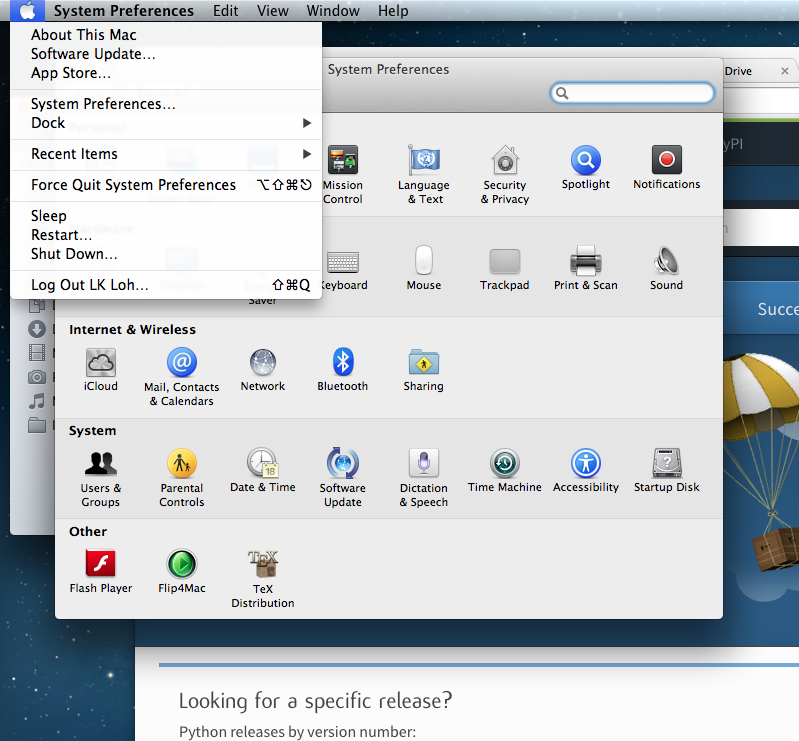
\includegraphics[width=0.5\textwidth]{images/system_preferences}
  \caption{Console}
  \label{fig:system_preferences}
\end{figure}

\begin{figure}[h!]
  \centering
  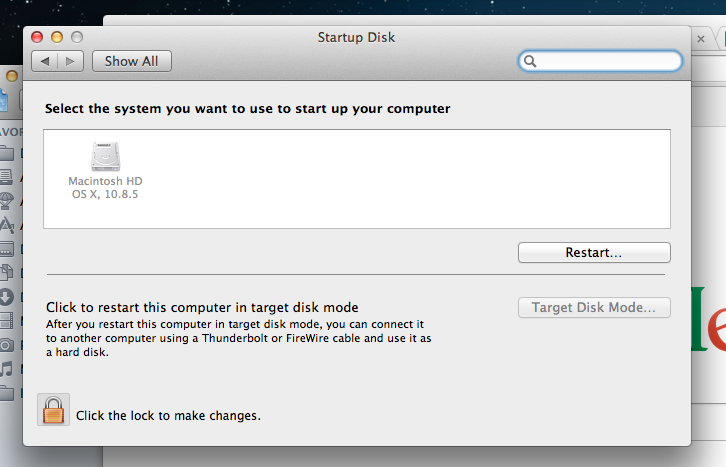
\includegraphics[width=0.5\textwidth]{images/startup_disk}
  \caption{Console}
  \label{fig:startup_disk}
\end{figure}

% ************************************************************* %
%                                                               %
%                       OPERATING SYSTEM                        %
%                                                               %
% ************************************************************* %

% ************************************************************* %
%                                                               %
%                       INSTALLING PYTHON                       %
%                                                               %
% ************************************************************* %

\section{Installing Python}

% ------------------------------------------------------------- %

\subsection{Getting Python}

Usually, Macs already have python installed by default. To check if you have python on your mac,
open up terminal, and do python in the terminal. If python is installed you should see some souch of console show up, as in Figure~\ref{fig:python_console}. If python is not installed, you should see an error message show up. 

\begin{figure}[h!]
  \centering
  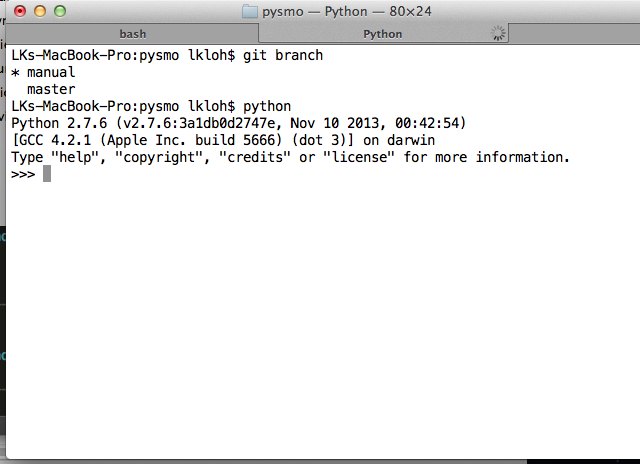
\includegraphics[width=0.5\textwidth]{images/python_console}
  \caption{Console}
  \label{fig:python_console}
\end{figure}

To get python, go to \url{https://www.python.org/}, and get the correct version for your operatin system. 

\begin{figure}[h!]
  \centering
  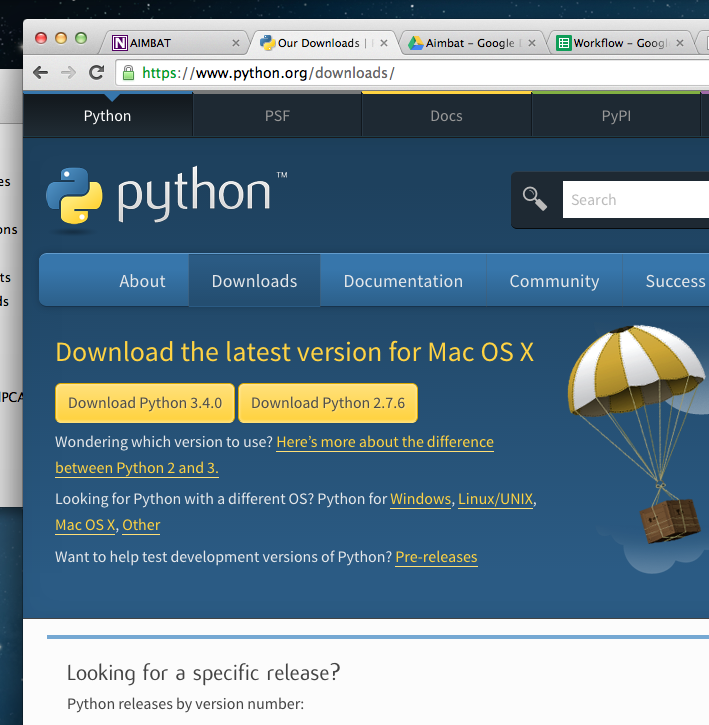
\includegraphics[width=0.5\textwidth]{images/python_version}
  \caption{Console}
  \label{fig:python_version}
\end{figure}

% ------------------------------------------------------------- %

\subsection{Macports}

Its best to use Macports \url{http://guide.macports.org/} to install the necessary python libraries for AIMBAT. 

If you just upgraded your operating system, you need to upgrade Macports and re-install the libraries as well. Follow the instructions here: \url{https://trac.macports.org/wiki/Migration}.

% ------------------------------------------------------------- %

\subsection{Installing the necessary components}

Inside the terminal, once python is install, type these commands in using sudo mode. Note you will need to enter your admin password.

\begin{verbatim}
  sudo port install python27
  sudo port install py27-numpy
  sudo port install py27-scipy
  sudo port install py27-matplotlib
  sudo port install py27-ipython
  sudo port install python_select
\end{verbatim}

Installing the last two packages is optional. \verb"ipython" is an enhanced interactive python shell.

\verb"python_select" is used to select default Python version by the following command:

\begin{verbatim}
  port select --set python python27
\end{verbatim}

You need this version, not other versions on your computer, since this is the one that has the libraries AIMBAT needs.

% ************************************************************* %
%                                                               %
%                       INSTALLING PYTHON                       %
%                                                               %
% ************************************************************* %

% ************************************************************* %
%                                                               %
%                       INSTALLING AIMBAT                       %
%                                                               %
% ************************************************************* %


\section{Installing AIMBAT}

% ------------------------------------------------------------- %

\subsection{Getting the packages}

AIMBAT is released as a sub-package of pysmo in the name of \verb"pysmo.aimbat" along with
another sub-package pysmo.sac. The latest releases of pysmo.sac and pysmo.aimbat are
available for download at \url{http://www.earth.northwestern.edu/~xlou/aimbat.html} and Github. 

The packages should be installed into the Python site-packages directory. To find out where that is, in the python console, do

\begin{verbatim}
  import site;
  site.getsitepackages()
\end{verbatim}

Whatever is output there, lets call it \verb"<pkg-install-dir>"

\begin{figure}[h!]
  \centering
  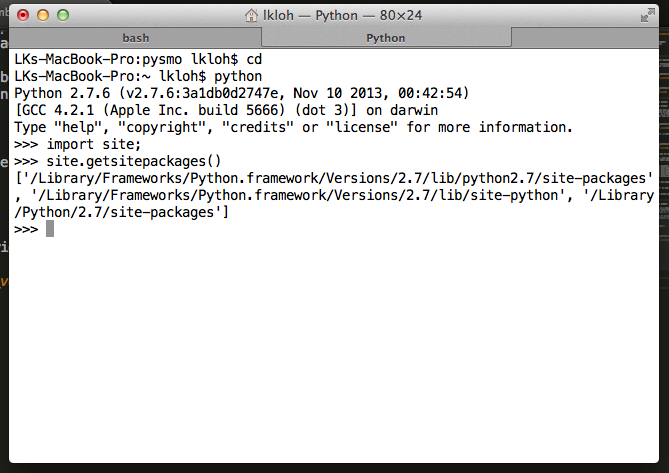
\includegraphics[width=0.5\textwidth]{images/site_package_location}
  \caption{Console}
  \label{fig:site_package_location}
\end{figure}

Now that we know the location of the site-packages direction, cd into it. Call the path to it \verb"<pkg-install-dir>" Notice that in this case, the site-packages has been installed for all users on the computer, not just the current user's home directory. 

Put the two Python packages inside the directory.

% -------------------------------------------------------------------------- %

\subsection{Installing pysmo.sac}

Python module \verb"Distutils" is used to write a setup.py script to build, distribute, and install \verb"pysmo.sac". In the directory \verb"<pkg-install-dir>/pysmo-sac-0.5>", type 

\begin{verbatim}
  python setup.py build
  python setup.py install
\end{verbatim}

to install it and its package information file \verb"<pysmo.sac-0.5-py2.7.egg-info" to the global site-packages directory \verb"<prefix>/lib/python2.7/site-packages", which is the same as Numpy, Scipy, and Matplotlib.

If you don't have write permission to the global site-packages directory, use the \verb"'--user'" option to install to \verb"<userbase>/lib/python2.7/site-packages":

\begin{verbatim}
  python setup.py install --user
\end{verbatim}

This will install it to your home directory only, not for all users on the computer. 

If you successfully installed the \verb"sac" module, in the python console, this should happen after you type \verb"from pysmo import sac": 

\begin{figure}[h!]
  \centering
  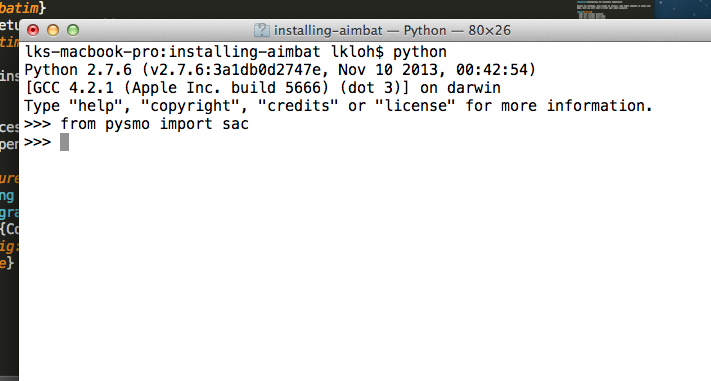
\includegraphics[width=0.5\textwidth]{images/sac_installed}
  \caption{Console}
  \label{fig:sac_installed}
\end{figure}

% ************************************************************* %
%                                                               %
%                       INSTALLING AIMBAT                       %
%                                                               %
% ************************************************************* %




















% ------------------------------------------------------------------------- %


\end{document}

% --------------------------------- END --------------------------------- %
